\documentclass[12pt,a4paper,oneside]{article}
\usepackage{graphicx,setspace,float,fancyhdr,listings,xcolor,placeins,xeCJK,tocloft,enumerate,amsmath,amssymb,bm}
\usepackage[dvipsnames]{xcolor}
\renewcommand{\cftsecleader}{\cftdotfill{\cftdotsep}} % Enable dot leaders in TOC
\renewcommand{\cftdotsep}{1} % Adjust dot spacing

\date{\Large 2024.12.21}
\author{陈海弘}

\setCJKmainfont[AutoFakeBold=3]{STFangsong} % CJK Font Setup
\setcounter{tocdepth}{3} % Set TOC depth
\setstretch{1.25} % Line spacing

% Page header and footer setup
\setlength{\headheight}{13.6pt}
\addtolength{\topmargin}{-1.6pt}
\pagestyle{fancy}
\fancyhf{}
\fancyhead[C]{\small Machine Learning} % Center header
\fancyfoot[C]{\small \thepage} % Center footer

% Code highlighting setup
\lstset{
    language=Python,
    basicstyle=\ttfamily\small,
    keywordstyle=\bfseries\color{NavyBlue},
    commentstyle=\itshape\color{red!50!green!50!blue!50},
    stringstyle=\bfseries\color{PineGreen!90!black},
    emph={self}, 
    emphstyle=\bfseries\color{Rhodamine},
    backgroundcolor=\color{black!3},
    frame=shadowbox,
    frameround=fttt,
    numbers=left,
    numberstyle=\tiny,
    stepnumber=1,
    numbersep=5pt,
    breaklines=true,
    columns=flexible,
    xleftmargin=1em,
    xrightmargin=-2em,
    aboveskip=1em,
    framexleftmargin=2em,
    escapeinside=``,
}

% Title setup
\title{
    \vspace*{-2cm}
    
\includegraphics[width=0.8\textwidth]{SYSULogo.pdf} \\[1em]
    \vfill
    \LARGE \textbf{机器学习实验报告6} \\[1em]
    \Large
    \begin{tabular}{rl}
        \textbf{姓名:} & \textbf{陈海弘} \\
        \textbf{学号:} & \textbf{23354049}
    \end{tabular}
    \vfill
}

\begin{document}

\maketitle
\newpage
\tableofcontents
\newpage
\section{摘要}
\qquad 本次实验主要是实现了ID3,C4.5,CART三种决策树算法,并且使用这三种算法对数据集进行分类。

最后做了一个决策树的实现,实现了决策树的生成和预测。
\section{前置准备}
本次实验包含的库有numpy,math,pandas,matplotlib,collections,counter.
\subsection{数据读取}
\qquad 本次实验使用的分类数据集中包含泰坦尼克号部分乘客的信息以及生还情况。数据集包括四个属性和一个标记属性,
Sex,SibSp,Parch,Pclass,Survived。数据集中已经没有缺失值和异常值,
所有连续变量已经离散化,标记属性Survived已经编码为0和1。读取部分代码过于简单,不再赘述。

\subsection{信息熵计算}
\qquad 计算信息熵公式:
某数组包含K个不同的取值,样本为第k(k=1,2,...,K)个值的数量所占比例为p\_k, 则其信息熵为$$Ent=-\sum_{k=1}^K p_k log_2 p_k$$

定义一个函数entropy,接受label数组,然后使用array将输入的数组转换为numpy,.flatten()将数组拉平,
使用unique函数找到不同的取值,然后统计每个唯一值在数组中出现的次数。
计算每一个counts的比例,最后用公式计算信息熵。

代码如下:
\begin{lstlisting}
def entropy(label):
    label = np.array(label).flatten()
    _, counts = np.unique(label, return_counts = True)
    pro = counts/counts.sum()
    ent = -np.sum(pro * np.log2(pro))
    return ent
\end{lstlisting}


结果如下:
\begin{figure}[H]
    \centering
    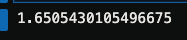
\includegraphics[width=0.3\textwidth]{image/1.png}
    \caption{信息熵计算}
\end{figure}

\subsection{维度划分}
\qquad 为了计算信息增益,需要将数据集按照某个属性划分为不同的子集。
函数将所给的数据集按照指定维度划分为若干个不同的数据集,输入属性集合、标记集合、维度索引,
输出划分后得到的子数属性集合,子树标记集合。子树属性集合就是按照维度划分后的数据集,子树标记集合是对应的标记集合。

给定一个特征矩阵 \texttt{feature}、标签数组 \texttt{label},以及划分维度 \texttt{dimension},该函数的目标是基于指定维度的特征值将数据划分为多个子集。具体思路如下:

\begin{enumerate}
    \item \textbf{输入处理:} \\
    将 \texttt{feature} 和 \texttt{label} 转换为 \texttt{NumPy} 数组,便于后续操作:
    \[
    \texttt{feature} \rightarrow \text{特征矩阵 (m $\times$ n)}, \quad
    \texttt{label} \rightarrow \text{标签向量 (m $\times$ 1)}
    \]

    \item \textbf{确定唯一值:} \\
    提取特征矩阵第 \texttt{dimension} 列的所有唯一值,表示在该维度上划分数据的类别:
    \[
    \texttt{unique\_values} = \texttt{np.unique(feature[:, dimension])}
    \]

    \item \textbf{初始化划分结果:} \\
    创建两个空列表,用于存储划分后的特征子集和对应的标签子集:
    \[
    \texttt{split\_feature} = [], \quad \texttt{split\_label} = []
    \]

    \item \textbf{按值划分数据:} \\
    对于每个唯一值 \texttt{value}:
    \begin{enumerate}
        \item 构造一个布尔掩码 \texttt{mask},筛选出 \texttt{feature} 中对应 \texttt{dimension} 列值等于 \texttt{value} 的行:
        \[
        \texttt{mask} = (\texttt{feature[:, dimension]} == \texttt{value})
        \]
        
        \item 根据掩码 \texttt{mask} 提取符合条件的特征子集和标签子集:
        \[
        \texttt{split\_feature.append(feature[mask].tolist())}
        \]
        \[
        \texttt{split\_label.append(label[mask].tolist())}
        \]
    \end{enumerate}

    \item \textbf{返回结果:} \\
    最终返回按 \texttt{dimension} 维度划分后的特征子集和标签子集:
    \[
    \texttt{return split\_feature, split\_label}
    \]
\end{enumerate}

代码如下:
\begin{lstlisting}
def split(feature, label, dimension):
    feature = np.array(feature)
    label = np.array(label)
    unique_values = np.unique(feature[:, dimension])
    split_feature = []
    split_label = []
    for value in unique_values:
        mask = feature[:,dimension] == value
        split_feature.append(feature[mask].tolist())
        split_label.append(label[mask].tolist())

    return split_feature,split_label
\end{lstlisting}

结果如下:
\begin{figure}[H]
    \centering
    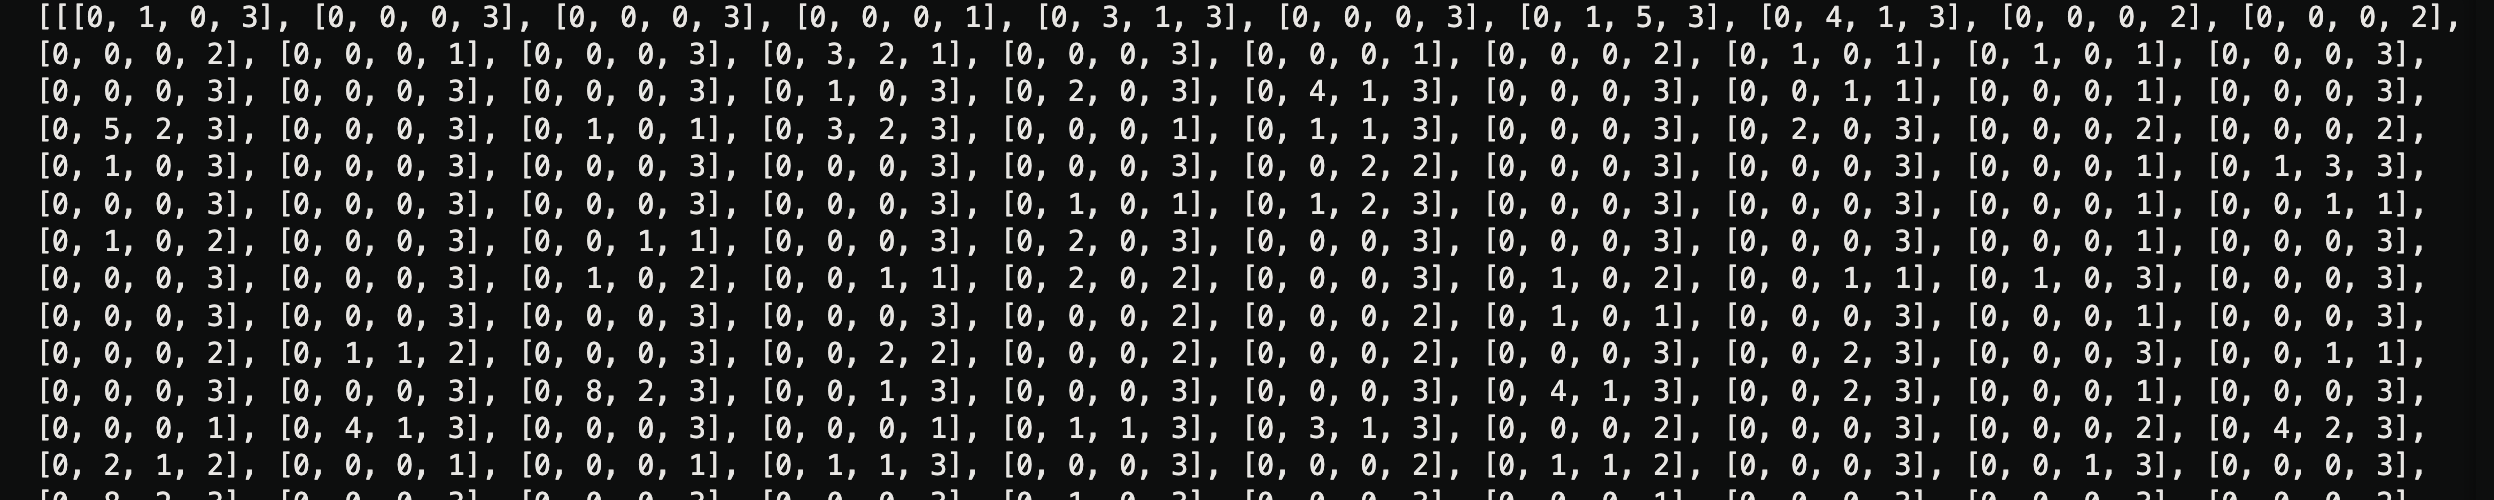
\includegraphics[width=0.7\textwidth]{image/2.png}
    \caption{属性集合}
\end{figure}

\begin{figure}[H]
    \centering
    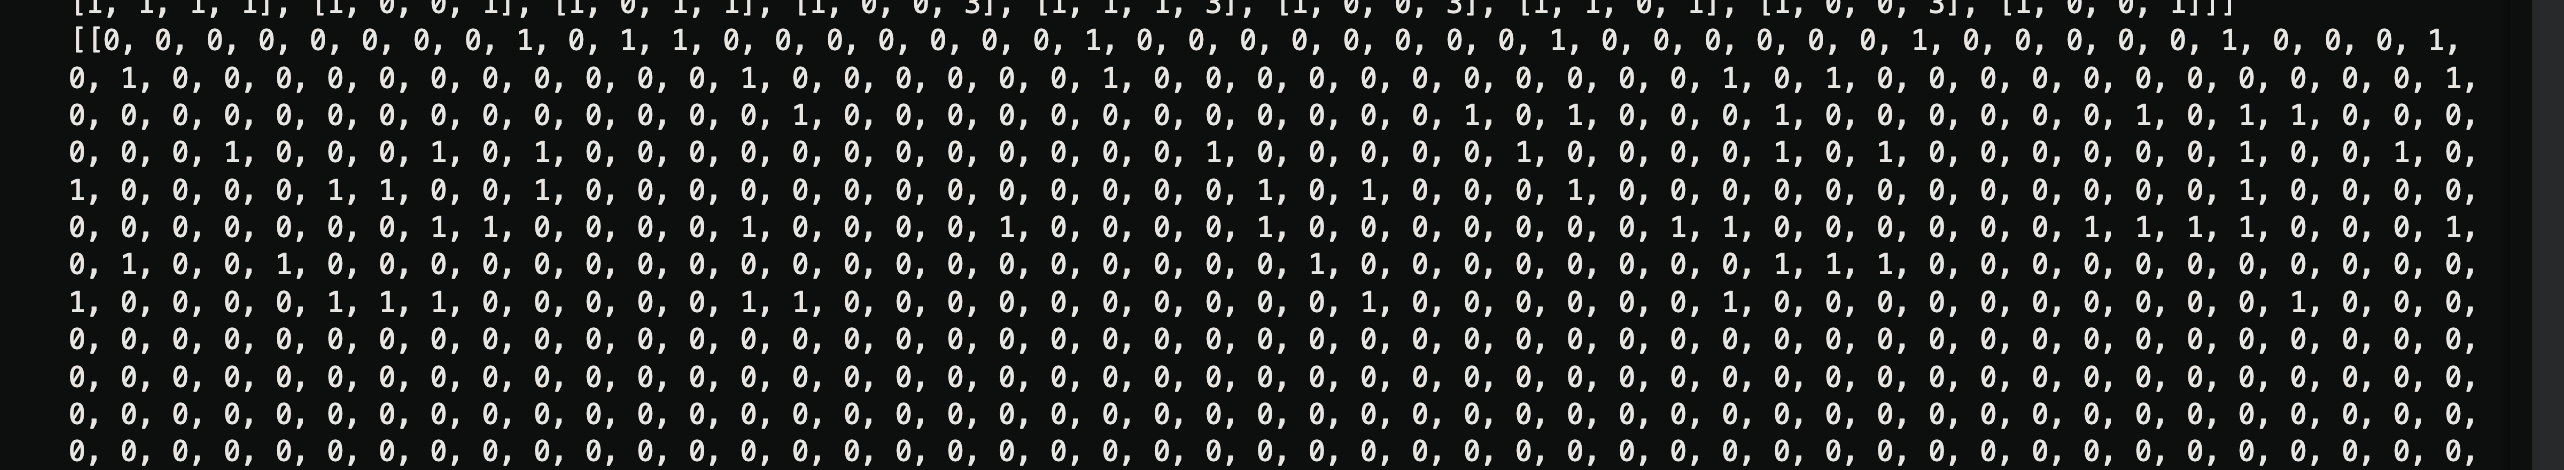
\includegraphics[width=0.7\textwidth]{image/3.png}
    \caption{标记集合}
\end{figure}

最后的属性集合和标记集合都是一个列表,列表中的元素是numpy数组,每个数组是一个子集。
可以看到,属性集合都是依据第一个维度划分的,分别是,0,1。标记集合就是对应的标记。
\section{ID3算法}
\qquad ID3算法就是使用信息增益来选择最优的属性进行划分,信息增益的计算公式如下:
$$Gain(D,A)=Ent(D)-\sum_{v=1}^V \frac{|D^v|}{|D|}Ent(D^v)$$

数据集D有属性值和标记值,样本总大小是|D|,属性A有V个不同的取值,
$D^v$是D中A属性取值为v的样本集合,$|D^v|$是$D^v$的大小,
Ent(D)是数据集D的信息熵,Ent($D^v$)是$D^v$的信息熵。

将特征矩阵 $\mathbf{X} \in \mathbb{R}^{n \times m}$ 
和标签向量 $\mathbf{y} \in \mathbb{R}^{n}$ 输入,
目标是找到最佳的特征维度 $d_{\text{best}}$,
以最大化信息增益 $G_{\text{best}}$。算法步骤如下:

1. 计算标签的总熵(Total Entropy):
   \[
   H_{\text{total}} = \text{Entropy}(\mathbf{y})
   \]

2. 初始化信息增益和分裂维度:
   \[
   G_{\text{best}} = -\infty, \quad d_{\text{best}} = -1
   \]

3. 遍历每一个特征维度 $d \in [1, 2, \ldots, m]$:
   - 按照维度 $d$ 对数据进行分裂,得到分裂后的特征和标签组:
     \[
     (\mathbf{X}_d^{\text{split}}, \mathbf{y}_d^{\text{split}})
     \]
   - 计算分裂后的条件熵(Conditional Entropy):
     \[
     H_{\text{conditional}} = \sum_{i} p_i \cdot \text{Entropy}(\mathbf{y}_i), \quad p_i = \frac{|\mathbf{y}_i|}{|\mathbf{y}|}
     \]
   - 计算信息增益(Information Gain):
     \[
     G = H_{\text{total}} - H_{\text{conditional}}
     \]
   - 如果 $G > G_{\text{best}}$,则更新:
     \[
     G_{\text{best}} = G, \quad d_{\text{best}} = d
     \]

4. 返回最佳信息增益和对应的分裂维度:
   \[
   \text{return } G_{\text{best}}, d_{\text{best}}
   \]

代码如下:
\begin{lstlisting}
def one_split_ID3(feature, label):
    feature = np.array(feature)
    label = np.array(label)
    n_features = feature.shape[1]
    total_entropy = entropy(label)
    
    best_gain = -np.inf
    best_dimension = -1

    for dim in range(n_features):
        split_feature, split_label = split(feature, label, dim)
        
        conditional_entropy = 0
        for labels in split_label:
            p = len(labels) / len(label)
            conditional_entropy += p * entropy(labels)
        
        gain = total_entropy - conditional_entropy
        
        if gain > best_gain:
            best_gain = gain
            best_dimension = dim

    return best_gain, best_dimension
\end{lstlisting}
\section{C4.5算法}
\qquad C4.5算法是ID3算法的改进版,使用信息增益率来选择最优的属性进行划分,信息增益率的计算公式如下:
$$GainRatio(D,A)=\frac{Gain(D,A)}{IV(A)}$$

将特征矩阵 $\mathbf{X} \in \mathbb{R}^{n \times m}$ 和标签向量 $\mathbf{y} \in \mathbb{R}^{n}$ 输入,目标是找到最佳的特征维度 $d_{\text{best}}$,以最大化信息增益率(Gain Ratio)。算法步骤如下:

1. 计算标签的总熵:
   \[
   H_{\text{total}} = \text{Entropy}(\mathbf{y})
   \]

2. 初始化:
   \[
   \text{最佳信息增益率 } G_{\text{best}} = -\infty, \quad \text{最佳维度 } d_{\text{best}} = -1
   \]

3. 遍历每个特征维度 $d \in [1, 2, \ldots, m]$:
   - 按照维度 $d$ 对数据进行分裂,得到分裂后的标签组 $\mathbf{y}_d^{\text{split}}$;
   - 计算分裂后的特征熵(Feature Entropy):
     \[
     H_{\text{feature}} = \sum_{i} \frac{|\mathbf{y}_i|}{|\mathbf{y}|} \cdot \text{Entropy}(\mathbf{y}_i)
     \]
     其中 $\mathbf{y}_i$ 是分裂后的子集标签。

   - 计算条件熵(Conditional Entropy):
     \[
     H_{\text{conditional}} = \sum_{i} \frac{|\mathbf{y}_i|}{|\mathbf{y}|} \cdot \text{Entropy}(\mathbf{y}_i)
     \]

   - 计算信息增益(Information Gain):
     \[
     G = H_{\text{total}} - H_{\text{conditional}}
     \]

   - 计算信息增益率(Gain Ratio):
     \[
     \text{如果 } H_{\text{feature}} \neq 0, \quad \text{Gain Ratio} = \frac{G}{H_{\text{feature}}}
     \]
     \[
     \text{否则,设 } \text{Gain Ratio} = 0
     \]

   - 如果当前维度的增益率大于历史最佳增益率:
     \[
     G_{\text{best}} = \text{Gain Ratio}, \quad d_{\text{best}} = d
     \]

4. 返回最佳信息增益率和对应的分裂维度:
   \[
   \text{return } G_{\text{best}}, d_{\text{best}}
   \]

代码展示:
\begin{lstlisting}  
    def one_split_C4_5(feature, label):
        feature = np.array(feature)
        label = np.array(label)
        n_features = feature.shape[1]
        total_entropy = entropy(label)
        
        best_gain_ratio = -np.inf
        best_dimension = -1
    
        for dim in range(n_features):
            split_feature, split_label = split(feature, label, dim)
            
            feature_entropy = 0
            total_size = len(label)
            for labels in split_label:
                feature_entropy += (len(labels) / total_size) * entropy(labels)
            
            conditional_entropy = 0
            for labels in split_label:
                p = len(labels) / len(label)
                conditional_entropy += p * entropy(labels)
            
            gain = total_entropy - conditional_entropy
            
            if feature_entropy != 0:
                gain_ratio = gain / feature_entropy
            else:
                gain_ratio = 0
            
            if gain_ratio > best_gain_ratio:
                best_gain_ratio = gain_ratio
                best_dimension = dim
    
        return best_gain_ratio, best_dimension
    
\end{lstlisting}
\section{CART算法}
CART算法是一种二叉树算法,使用基尼指数来选择最优的属性进行划分,基尼指数的计算公式如下:
$$Gini(D)=1-\sum_{k=1}^K p_k^2$$
每一个属性的基尼指数是:
$$Gini(D,A)=\sum_{v=1}^V \frac{|D^v|}{|D|}Gini(D^v)$$

将特征矩阵 $\mathbf{X} \in \mathbb{R}^{n \times m}$ 和标签向量 $\mathbf{y} \in \mathbb{R}^{n}$ 输入,目标是找到最佳的特征维度 $d_{\text{best}}$ 和分裂值 $v_{\text{best}}$,以最小化基尼指数(Gini Index)。算法步骤如下:

1. 初始化:
   \[
   \text{最佳基尼指数 } G_{\text{best}} = \infty, \quad \text{最佳维度 } d_{\text{best}} = -1, \quad \text{最佳划分值 } v_{\text{best}} = \text{None}
   \]

2. 遍历每个特征维度 $d \in [1, 2, \ldots, m]$:
   - 找到当前特征的所有唯一值(Unique Values):
     \[
     \text{unique\_values} = \text{Unique}(\mathbf{X}[:, d])
     \]

   - 遍历每个唯一值 $v \in \text{unique\_values}$:
     - 按照 $v$ 将数据分为两个子集:
       \[
       \text{左子集: } \mathbf{X}_{\text{left}}, \mathbf{y}_{\text{left}} \quad \text{其中 } \mathbf{X}[:, d] \leq v
       \]
       \[
       \text{右子集: } \mathbf{X}_{\text{right}}, \mathbf{y}_{\text{right}} \quad \text{其中 } \mathbf{X}[:, d] > v
       \]

     - 计算两个子集的基尼系数:
       \[
       G_{\text{left}} = 1 - \sum_{c} \left( \frac{\text{count}(c, \mathbf{y}_{\text{left}})}{|\mathbf{y}_{\text{left}}|} \right)^2
       \]
       \[
       G_{\text{right}} = 1 - \sum_{c} \left( \frac{\text{count}(c, \mathbf{y}_{\text{right}})}{|\mathbf{y}_{\text{right}}|} \right)^2
       \]

     - 计算当前划分的加权基尼指数:
       \[
       G_{\text{index}} = \frac{|\mathbf{y}_{\text{left}}|}{|\mathbf{y}|} G_{\text{left}} + \frac{|\mathbf{y}_{\text{right}}|}{|\mathbf{y}|} G_{\text{right}}
       \]

     - 如果 $G_{\text{index}} < G_{\text{best}}$,则更新最佳基尼指数及对应的维度和划分值:
       \[
       G_{\text{best}} = G_{\text{index}}, \quad d_{\text{best}} = d, \quad v_{\text{best}} = v
       \]

3. 返回最佳基尼指数、最佳分裂维度和分裂值:
   \[
   \text{return } G_{\text{best}}, d_{\text{best}}, v_{\text{best}}
   \]

代码展示:
\begin{lstlisting}
    def gini(labels):
        total_size = len(labels)
        if total_size == 0:
            return 0
        label_counts = Counter(labels)
        gini_score = 1 - sum((count / total_size) ** 2 for count in label_counts.values())
        return gini_score
    def one_split_CART(feature, label):
        feature = np.array(feature)
        label = np.array(label)
        n_features = feature.shape[1]
        
        best_gini = np.inf
        best_dimension = -1
        best_value = None
    
        for dim in range(n_features):
            unique_values = np.unique(feature[:, dim])  # 找到每列的非重复值
            
            for value in unique_values:
                # 按当前特征值将数据划分为两个子集
                left_indices = feature[:, dim] <= value
                right_indices = feature[:, dim] > value
                
                left_labels = label[left_indices]
                right_labels = label[right_indices]
                
                # 计算子集的基尼系数
                left_gini = gini(left_labels)
                right_gini = gini(right_labels)
                total_size = len(label)
                
                gini_index = (len(left_labels) / total_size) * left_gini + \
                             (len(right_labels) / total_size) * right_gini
                
                # 更新最小基尼系数及对应的维度和划分值
                if gini_index < best_gini:
                    best_gini = gini_index
                    best_dimension = dim
                    best_value = value
    
        return best_gini, best_dimension, best_value
\end{lstlisting}

\section{实验结果}
\begin{figure}[H]
    \centering
    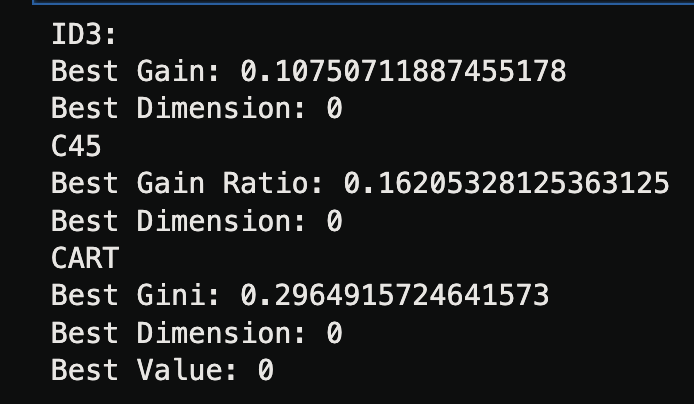
\includegraphics[width=0.7\textwidth]{image/4.png}
    \caption{结果展示}
\end{figure}
\qquad 结果可以看出,这三个算法的结果算出的最佳维度都是0,ID3算出的最佳增益是0.107,
C4.5算出的最佳增益率是0.16,CART算出的最佳基尼指数是0.29,对应的分类值是0。

\section{决策树}
\qquad 这里用ID3算法实现决策树,完成DTree类中的Tree Generate,
train函数以完成决策树的构建,并用构建好的决策树来对测试数据集进行预测并输出结果。



ID3算法的核心思想是通过计算信息增益来选择最优属性,并根据该属性划分数据集。具体的构建过程如下:

\begin{enumerate}
    \item \textbf{初始化:}
    通过传入的数据集$D$,首先确定每个属性的可能取值,并初始化决策树的根节点。在代码中,这通过`self.possible\_value`字典来实现:
    \[
    \text{self.possible\_value[attr]} = \text{np.unique}(D[:, attr])
    \]
    这一步为每个属性记录其可能的取值。数据集$D$的最后一列为标签列,表示每个样本的类别。`D[:, -1]`表示提取标签列。
    
    \item \textbf{计算信息熵:}
    信息熵$H(D)$用于衡量数据集$D$的不确定性。其公式为:
    \[
    H(D) = -\sum_{i} p_i \log_2 p_i
    \]
    其中$p_i$为类别$i$在数据集$D$中出现的概率。在代码中,信息熵通过`entropy`方法计算,利用`np.unique`统计不同类别的频次:
    \[
    \text{labels, counts} = \text{np.unique}(D[:, -1], \text{return\_counts=True})
    \]
    然后计算熵值:
    \[
    H(D) = -\sum \left(\frac{\text{count}}{\text{total}} \times \log_2 \left(\frac{\text{count}}{\text{total}}\right)\right)
    \]
    这里`total`是数据集$D$的样本总数。

    \item \textbf{计算信息增益:}
    对于每个属性,计算该属性的信息增益。信息增益$IG$表示使用该属性划分数据集后,信息熵的减少量。信息增益的公式为:
    \[
    IG(D, A) = H(D) - H(D|A)
    \]
    其中$H(D|A)$是数据集$D$在属性$A$上的条件熵,表示在属性$A$的每个可能取值下数据集$D$的熵的加权平均。代码中,`info\_gain`方法计算了信息增益:
    \[
    \text{total\_entropy} = \text{self.entropy}(D)
    \]
    然后对于每个属性的每个取值,计算条件熵并累加:
    \[
    \text{conditional\_entropy} = \sum \left( \frac{\text{counts}[i]}{\text{total}} \times \text{self.entropy}(D[D[:, \text{attr\_index}] == \text{values}[i]]) \right)
    \]
    最终,信息增益为总熵减去条件熵:
    \[
    \text{info\_gain} = \text{total\_entropy} - \text{conditional\_entropy}
    \]

    \item \textbf{选择最优属性:}
    对于当前数据集$D$,选择信息增益最大的属性作为划分的标准。代码中通过以下方式选择最优属性:
    \[
    \text{best\_attr} = \max(A, \text{key}=\lambda \text{attr}: \text{self.info\_gain}(D, \text{attr}))
    \]
    如果信息增益为零或所有样本在某属性上的取值相同,则停止划分并将当前节点标记为叶子节点,赋值为样本类别中最多的类别。具体地,在`TreeGenerate`方法中,若所有样本类别相同,则创建一个叶节点并返回:
    \[
    \text{node.isLeaf} = \text{True}, \quad \text{node.label} = \text{unique\_labels}[0]
    \]

    \item \textbf{递归构建子树:}
    对于选定的最优属性,将数据集$D$按该属性的取值进行划分。然后,对于每个划分得到的子集,递归地进行相同的操作。代码中,对每个子集递归地调用`TreeGenerate`方法:
    \[
    \text{subset} = D[D[:, \text{best\_attr}] == \text{value}]
    \]
    对每个子集,递归调用:
    \[
    \text{child\_node} = \text{self.TreeGenerate}(\text{subset}, A - \{\text{best\_attr}\})
    \]
    直到所有子集中的样本属于同一类别,或没有可用的属性进行划分。若子集为空,则创建一个叶节点,并选择出现次数最多的类别作为标签:
    \[
    \text{child\_node} = \text{Node}(isLeaf=\text{True}, label=\text{unique\_labels}[\text{np.argmax}(counts)])
    \]

    \item \textbf{预测:}
    对于每个待预测样本,根据构建好的决策树,从根节点开始沿着属性的取值进行遍历,最终到达叶子节点,叶子节点的标签即为预测结果。代码中,通过递归遍历决策树实现预测:
    \[
    \text{node} = \text{self.tree\_root}
    \]
    对每个样本,沿着决策树的分支进行判断,直到到达叶节点:
    \[
    \text{attr\_value} = \text{data[node.index]}
    \]
    最终,通过比较预测值与真实标签,计算准确率:
    \[
    \text{accuracy} = \frac{\text{correct}}{\text{total}}
    \]
\end{enumerate}

代码展示:
\begin{lstlisting}
  class DTree:
  def __init__(self):
      self.tree_root = None  
      self.possible_value = {}  

  def entropy(self, D):
      labels, counts = np.unique(D[:, -1], return_counts=True)
      total = len(D)
      return -sum((count / total) * math.log2(count / total) for count in counts)

  def info_gain(self, D, attr_index):
      total_entropy = self.entropy(D)
      values, counts = np.unique(D[:, attr_index], return_counts=True)
      total = len(D)
      conditional_entropy = sum((counts[i] / total) * self.entropy(D[D[:, attr_index] == values[i]])
                                 for i in range(len(values)))
      return total_entropy - conditional_entropy

  def TreeGenerate(self, D, A):
      node = Node()
      labels = D[:, -1]
      unique_labels, counts = np.unique(labels, return_counts=True)

      if len(unique_labels) == 1:
          node.isLeaf = True
          node.label = unique_labels[0]
          return node

      if len(A) == 0 or all(np.all(D[:, a] == D[0, a]) for a in A):
          node.isLeaf = True
          node.label = unique_labels[np.argmax(counts)] 
          return node

      best_attr = max(A, key=lambda attr: self.info_gain(D, attr))
      node.isLeaf = False
      node.index = best_attr

      for value in self.possible_value[best_attr]:
          subset = D[D[:, best_attr] == value]
          if len(subset) == 0:  
              child_node = Node(isLeaf=True, label=unique_labels[np.argmax(counts)])
          else:
              remaining_attrs = A - {best_attr}
              child_node = self.TreeGenerate(subset, remaining_attrs)
          node.addNode(value, child_node)
      
      return node

  def train(self, D):
      D = np.array(D)  
      A = set(range(D.shape[1] - 1)) 
      for attr in A:
          self.possible_value[attr] = np.unique(D[:, attr]) 
      self.tree_root = self.TreeGenerate(D, A)  

  def predict(self, D):
      D = np.array(D)  
      correct = 0
      total = len(D)
      
      for data in D:
          node = self.tree_root
          while not node.isLeaf:  
              attr_value = data[node.index]
              if attr_value in node.children:
                  node = node.children[attr_value]
              else: 
                  node = Node(isLeaf=True, label=-1)  
          
          if node.label == data[-1]:  
              correct += 1
      
      accuracy = correct / total
      print(f"Accuracy: {accuracy:.2f}")
\end{lstlisting}

结果展示:
\begin{figure}[H]
    \centering
    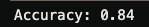
\includegraphics[width=0.3\textwidth]{image/5}
    \caption{决策树结果}
\end{figure}
最后的结果是0.84,说明决策树的准确率还是不错的。

\section{总结}
\qquad 这次实验主要实现了三种决策树算法,ID3,C4.5,CART,然后实现了一个决策树的生成和预测。

ID3算法的好处是简单,易于理解,但是缺点是容易过拟合,不能处理连续值,C4.5算法是ID3的改进版,
可以处理连续值,但是C4.5算法对于缺失值的处理不是很好,
CART算法是一种二叉树算法,可以处理连续值和缺失值,但是CART算法的结果是二叉树,不是多叉树。

对于数据处理的时候,需要对数据进行预处理,将连续值离散化,将缺失值填充,将标签编码,这是我容易遗忘的。
\end{document}